\documentclass[t,landscape]{beamer}
%\documentclass[handout]{beamer}

\mode<presentation> { \usetheme{PaloAlto} }

\usepackage[latin1]{inputenc}
\title[Accumulo]{Accumulo: NoSQL Database}
\author[]{David Medinets\\Eclectic Consulting\\ \texttt{http://www.codebits.com} \\ \texttt{david.medinets@gmail.com} \\ Fairfax, VA}
\institute{XLDB 2012}
\date{September 2012}

\usepackage{amsmath}
\usepackage{graphicx}

\newcommand{\ampersand}{\mathbin{\&}}

\AtBeginSection[]
{
  \begin{frame}{Progress}
    \tableofcontents[currentsection]
  \end{frame}
}

\AtBeginSubsection[] 
{ 
  \begin{frame}{Progress}
    \tableofcontents[currentsection,currentsubsection] 
  \end{frame} 
}

\begin{document}

% Add the label current to a frame and uncomment the
% following line to speed up the make process.
%\includeonlyframes{current}

\begin{frame}
\titlepage
\end{frame}

\begin{frame}{Contents}
\tableofcontents
\end{frame}

\section{Introduction}
\begin{frame}{What is Accumulo?}
\begin{itemize}
\item{}
\item{Self-alone system. This laptop is weak.}
\item{Discussing and demonstrating v1.5.0}
\end{itemize}
\end{frame}

\begin{frame}{Background Information}
\begin{center}

\includegraphics[width=0.4\textwidth]{images/accumulo-logo.png}
\end{center}
\scriptsize
\begin{itemize}
\item{First code written in Spring of 2008}
\item{Open-sourced as an Apache Software Foundation incubator podling in September, 2011}
\item{Graduated to Top-Level Project in March, 2012}
\item{Mostly a clone of Bigtable, but includes several notable features:
	\begin{itemize}
		\scriptsize
		\item{Iterators: a framework for processing sorted streams of key/value entries}
		\item{Cell-level Security: mandatory, attribute-based access control with key/value granularity}
		%\item{Isolation for large rows}
		\item{Fault-Tolerant Execution Framework (FATE)}
		\item{A compaction scheduler with nice properties}
	\end{itemize}
% TODO most importantly, we learned alot (include graphic) about distributed computing in the process
}
\end{itemize}
\end{frame}
\note{NSA started experimenting with Hadoop in 2007, and quickly realized the need for a Bigtable-like system.}
\note{After evaluating early versions of several open-source Bigtable clones, NSA decided to write their own version.}
\note{This was primarily for stability, write performance, and scalability concerns.}
\note{After several iterations we have settled on a couple of frameworks that have drastically simplified the code base: Iterators and FATE.}

\begin{frame}{Accumulo around the web}
- Accumulo user group on meetup.com, Sqrrl, Twitter feed, A. Cordova
\end{frame}

\begin{frame}{Shell}
\begin{itemize}
  \scriptsize
  \item{Debugging: classpath, debug, listscans, trace}
  \item{Exiting: bye, quit, exit}
  \item{Help: about, help, info, ?}
  \item{Iterator: deleteiter, deletescaniter, listiter, setiter, setscaniter}
  \item{Permission Admin: grant, revoke, systempermissions, tablepermissions, userpermissions}
  \item{Execution: execfile, history}
  \item{Shell State: authenticate, cls, clear, notable, sleep, table, user, whoami}
  \item{Table Admin: clonetable, config, createtable, deletetable, droptable, du, offline, online, renametable, tables}
  \item{Table Control: addsplits, compact, constraint, flush, getgroups, getsplits, merge, setgroups}
  \item{User Admin: createuser, deleteuser, dropuser, getauths, passwd, setauths, users}
  \item{Data: delete, deletemany, deleterows, egrep, formatter, grep, importdirectory, insert, maxrow, scan}
\end{itemize}
\end{frame}

\begin{frame}{Monitor Page}
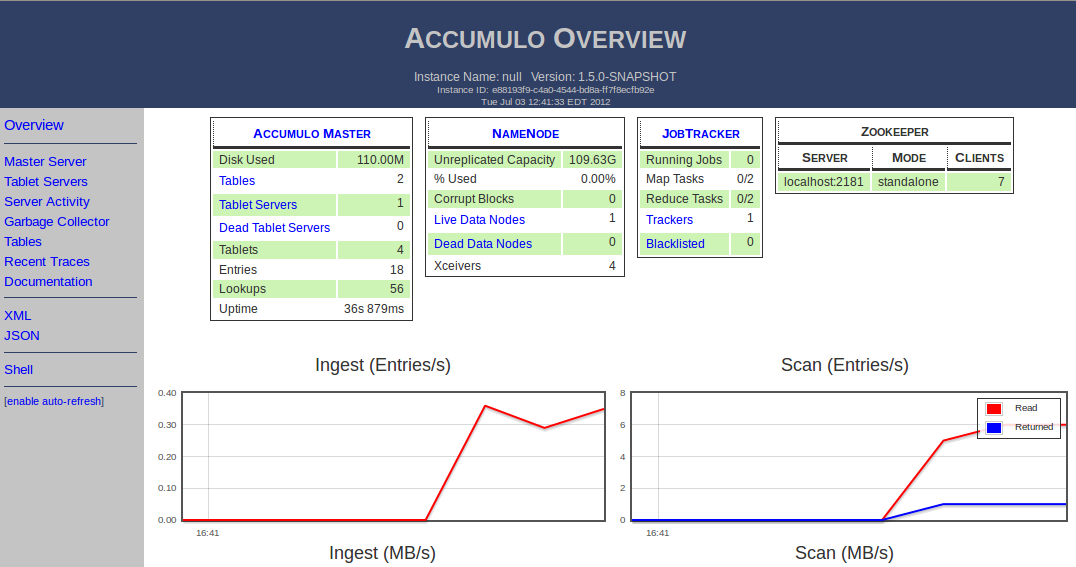
\includegraphics[width=0.75\textwidth]{images/accumulo_monitor_page.png}
\begin{itemize}
\item{Information can be pulled as XML or JSON for monitoring programs like ganglia or nagios.}
\item{HTTPS is supported.}
\end{itemize}
\end{frame}

\begin{frame}{Other Features}
\scriptsize
Check out Apache Accumulo (\textcolor{blue}{http://accumulo.apache.org/}) for interesting implementations of:
\begin{itemize}
\item{Merging Tablets}
\item{Table Cloning: Hard link-style table copying}
\item{Relative Key Encoded RFile file format}
\item{Adaptive locality groups}
\item{Isolation over scans of wide rows}
\item{Bulk loading}
\item{Logical time}
\item{Client-side threading models for batch writes and scans}
\item{Merging minor compactions}
\item{Distributed write-ahead log}
\end{itemize}
\end{frame}

\begin{frame}[label=current]{Key is a 5-tuple}
An Accumulo Key is a 5-tuple, including:
\begin{itemize}
  \item{\textbf{Row}: controls \emph{Atomicity}}
  \item{\textbf{Column Family}: controls \emph{Locality}}
  \item{\textbf{Column Qualifier}: controls \emph{Uniqueness}}
  \item{\textbf{Visibility}: controls \emph{Access} (unique to Accumulo)}
  \item{\textbf{Timestamp}: controls \emph{Versioning}}
\end{itemize}

\begin{block}{Sample Entries}
\tiny
\begin{tabular}{llllll}
Row &: Col. Fam. &: Col. Qual. &: Visibility &: Timestamp & $\Rightarrow$ Value \\\hline
Adam &: Favorites &: Food &: (Public) &: 20090801 &$\Rightarrow$ Sushi \\
Adam &: Favorites &: Programming Language &: (Private) &: 20090830 &$\Rightarrow$ Java \\
Adam &: Favorites &: Programming Language &: (Private) &: 20070725 &$\Rightarrow$ C++ \\
Adam &: Friends &: Bob &: (Public) &: 20110601 & $\Rightarrow$ \\
Adam &: Friends &: Joe &: (Private) &: 20110601 & $\Rightarrow$ \\
\end{tabular}
\end{block}
\note{The last two entries has no value. This is a common design pattern.}
\end{frame}

\begin{frame}{Values are bytes}
bytes are bytes (images, text, whatever.)
\end{frame}

\begin{frame}{Physical Data Model}
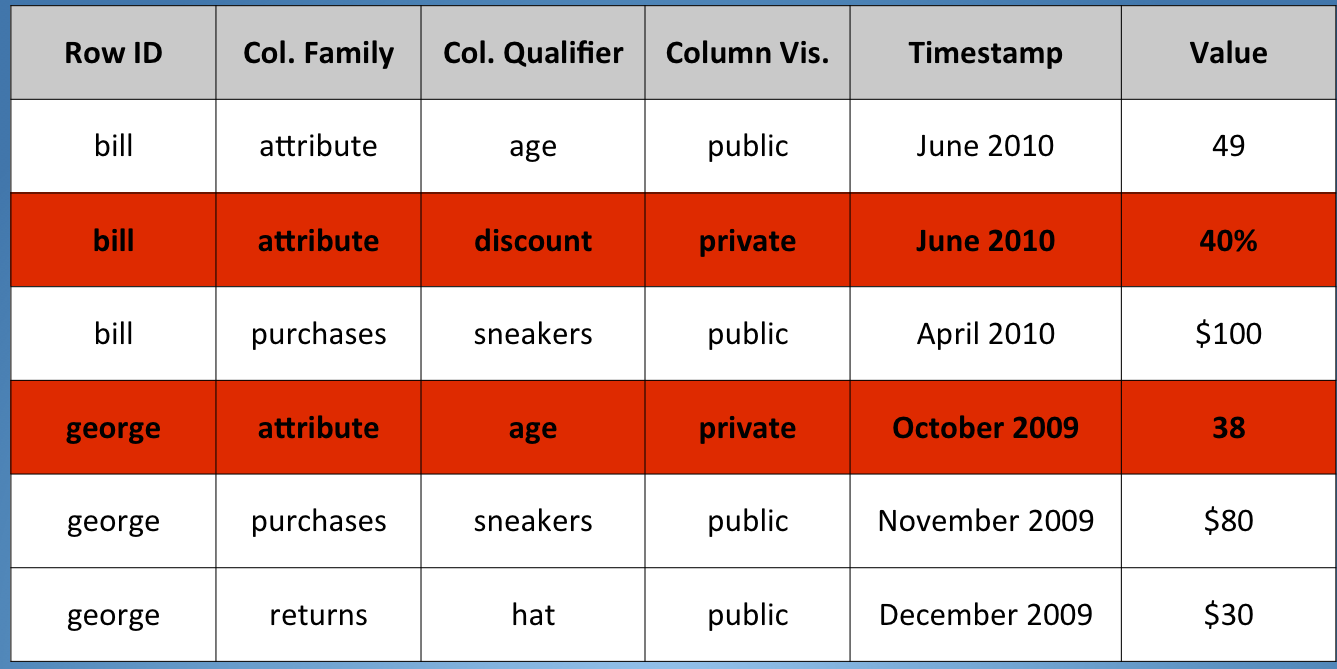
\includegraphics[width=\textwidth]{images/physical_data_model_dmm.png}
\end{frame}

\begin{frame}{RDBS Representation}
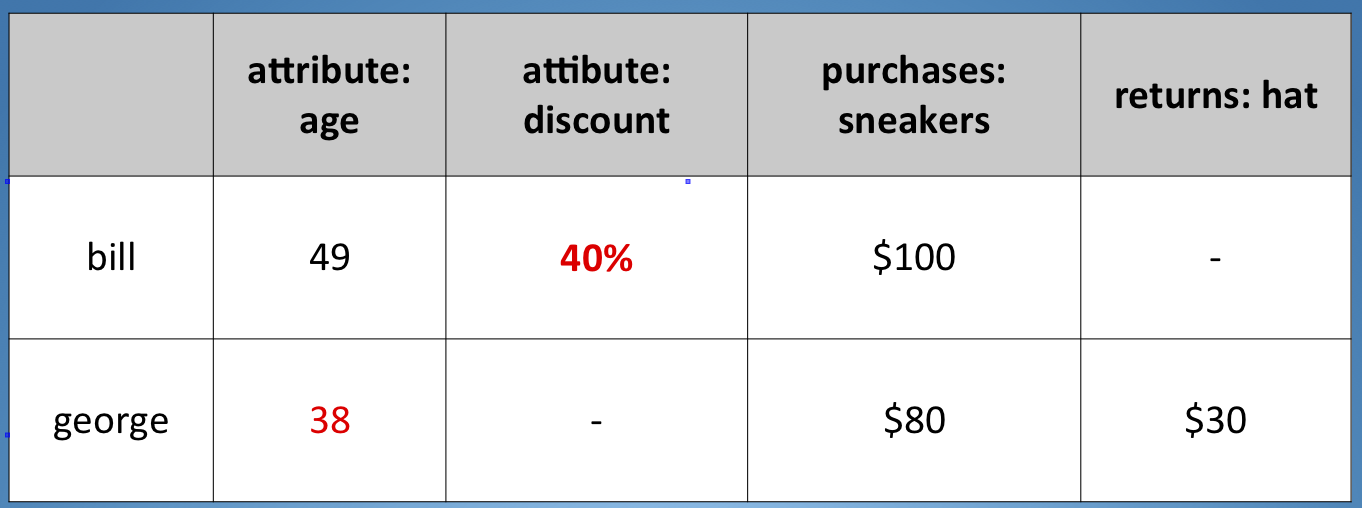
\includegraphics[width=\textwidth]{images/2d_table_layout_dmm.png}
\begin{block}{Note}
Column visibility (i.e., public vs private) is not supported.
\end{block}
\end{frame}

\begin{frame}{Hierarchical Decomposition}
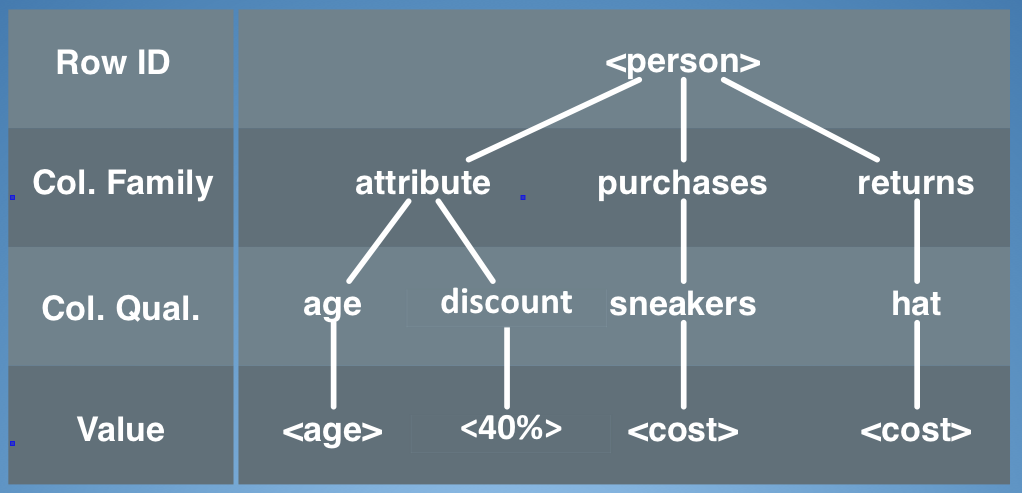
\includegraphics[width=\textwidth]{images/hierarchical_decomposition_dmm.png}
\begin{block}{Note}
Depiction of NoSQL schemas is not easy. Value placeholders are shown here.
\end{block}
\end{frame}

\begin{frame}{Hierarchical Representation}
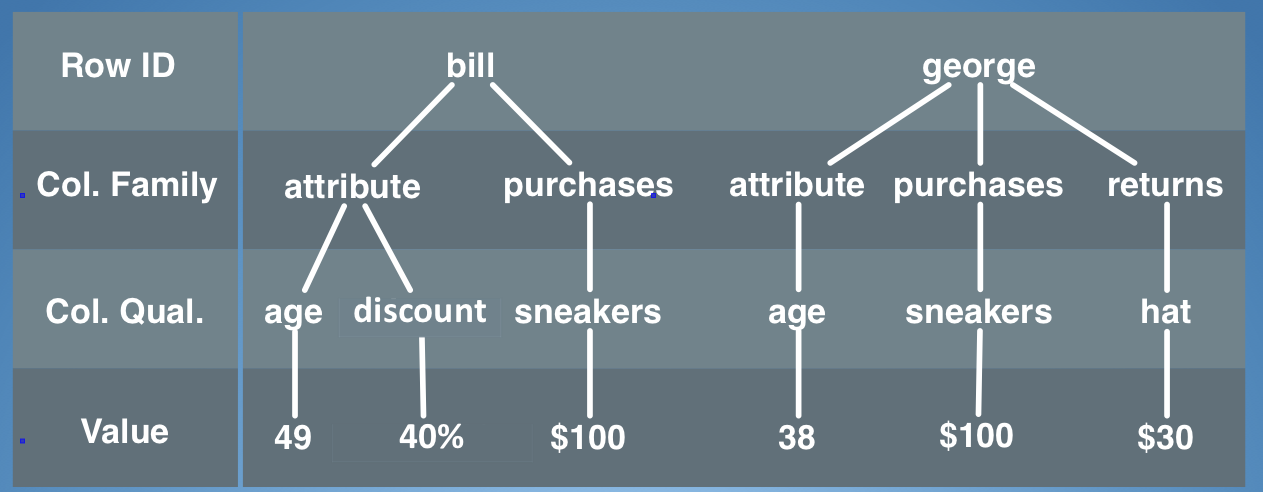
\includegraphics[width=\textwidth]{images/concrete_hierarchical_decomposition_dmm.png}
\begin{block}{Note}
The actual values are shown here.
\end{block}
\end{frame}

\begin{frame}[fragile]{Creating Records With Labels}
\begin{verbatim}
createtable demo
insert bill   attribute age      -l public  49
insert bill   attribute discount -l private .40
insert bill   purchases sneakers -l public  100.00
insert george attribute age      -l private 38
insert george purchases sneakers -l public  80.00
insert george returns   hat      -l public  30.00
\end{verbatim}
\end{frame}

\begin{frame}[fragile]{User With One Authorization}
\begin{verbatim}
scan
# no results
setauths -s public -u root
scan
 bill attribute:age [public]    49
 bill purchases:sneakers [public]    100.00
 george purchases:sneakers [public]    80.00
 george returns:hat [public]    30.00
setauths -s private -u root
scan
 bill attribute:discount [private]    .40
 george attribute:age [private]    38
\end{verbatim}
\end{frame}

\begin{frame}[fragile]{User With Multiple Authorizations}
\begin{verbatim}
setauths -s public,private -u root
scan
 bill attribute:age [public]    49
 bill attribute:discount [private]    .40
 bill purchases:sneakers [public]    100.00
 george attribute:age [private]    38
 george purchases:sneakers [public]    80.00
 george returns:hat [public]    30.00
\end{verbatim}
\end{frame}

\begin{frame}{Tablet description}
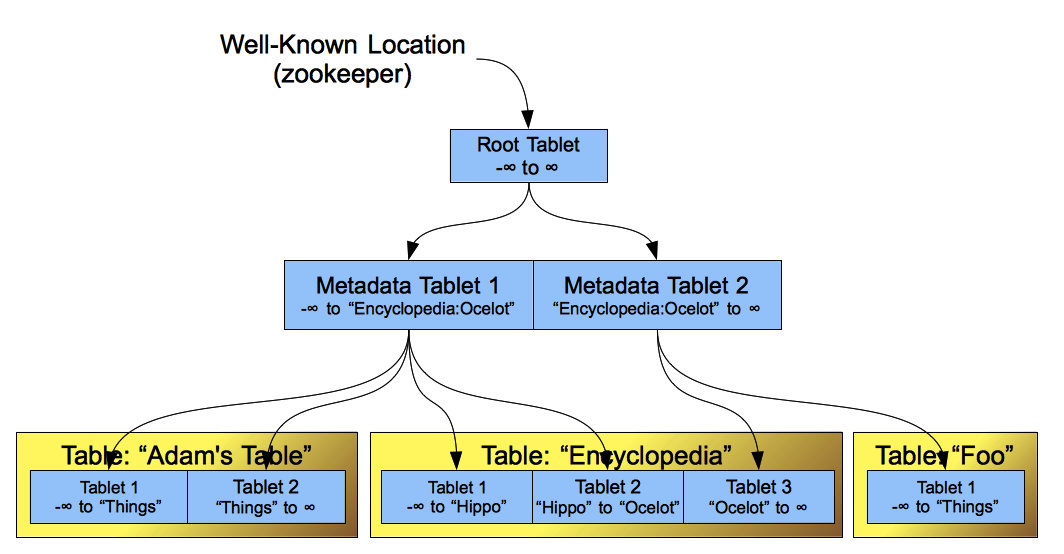
\includegraphics[width=\textwidth]{images/tablet_organization.png}
\begin{itemize}
\item{Tables are just another grouping mechanism,}
\item{Metadata tablets hold info about other tablets, forming a three-level hierarchy}
\end{itemize}
\end{frame}

\begin{frame}{Tablet Server Data Flow}
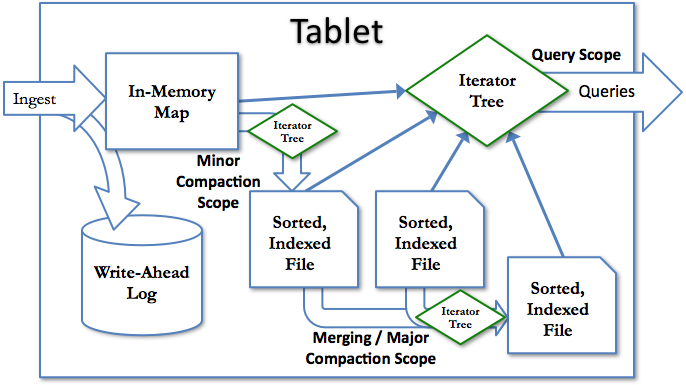
\includegraphics[width=0.9\textwidth]{images/tablet_flow.png}
\begin{itemize}
\item{Minor compaction - a new in-memory map and a new file replace the old in-memory map}
\item{Major compaction - a new file replaces some subset of the old files}
\end{itemize}
\end{frame}
\note{The diagram shows data flow within a tablet server on behalf of a tablet.}
\note{Tablets are primarily concerned with ingest (randomly ordered key/value pairs), and query (sequentially ordered ranges of key/value pairs).}
\note{This data flow forms a log-structure merge tree.}
\note{All Files and the In-Memory Map are sorted locally, but may overlap each other in range. Queries often need to stream data merged from multiple files and the in-memory map.}

\section{Iterators}

\begin{frame}{What is an Iterator?}
\begin{itemize}
\item{An \emph{Iterator} provides an ordered stream of key/value pairs, and supports basic \emph{selection} and \emph{filtering} methods.}
\item{Iterators are executed at three points:}
\begin{itemize}
\item{Scan - query time}
\item{Minor Compaction - in-memory to file}
\item{Major Compaction - merging files}
\end{itemize}
\end{itemize}
\end{frame}

\begin{frame}{An Example of Summing Combining Aggregation}
  \begin{center}
  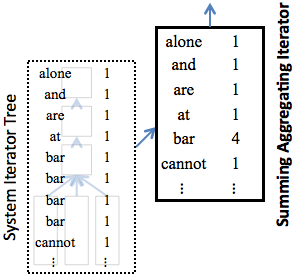
\includegraphics[width=0.6\textwidth]{images/aggregator.png}
  \end{center}
  \begin{itemize}
    \item{Any associative, commutative operations can be encoded in an aggregator}
    \item{Aggregators can persist an aggregation of the entries written to the table}
    \item{Aggregators are efficient due to lazy aggregation}
  \end{itemize}
\end{frame}

% MS24
\begin{frame}
\frametitle{Multi-Term Query with Document Partitioning}

\begin{center}

\normalsize
Goal: Find all of the documents that contain \\ the words ``foo" and ``bar".

\scriptsize
\begin{block}{Partitioned Corpus}
\begin{tabular}{ll}
	$\left.
	\mbox{
	\begin{tabular}{ll}
		$Doc_1 :$
			& $\texttt{\scriptsize"foo and bar are common variable names"}$ \\
		$Doc_2 :$
			& $\texttt{\scriptsize"one cannot live on bar food alone"}$ \\
		$Doc_3 :$
			& $\texttt{\scriptsize"Mr.\noindent T pities the fool at the bar"}$
	\end{tabular}
	}
	\right\}$
			&$Partition_1$\\

	$\left.
	\mbox{
	\begin{tabular}{ll}
		$Doc_4 :$
			& $\texttt{\scriptsize"someone should invent the kung foo bar"}$
	\end{tabular}
	}
	\right\}$
			&$Partition_2$
\end{tabular}
\end{block}
\end{center}
\end{frame}

%%%%%%%%%%%%%%%%%%%%%%%%%%%%%%%%%%%%%%%%%%%%%%%%%%%%%%%%
% document partitioned table example for intersecting iterator

% MS25
\begin{frame}
\frametitle{Document Partitioning}
\begin{center}
\small
Divide and Conquer:

\normalsize
\begin{minipage}{0.35\textwidth}
\begin{center}
\begin{picture}(225,0)
\put(0,-78){\dashbox{3}(100,7){}}
\put(0,-57){\dashbox{3}(100,21){}}
\put(106,-57){\dashbox{3}(100,7){}}
\put(106,-64){\dashbox{3}(100,7){}}
\end{picture}
\tiny
\begin{tabular}{|lll|}\hline
Row&ColFam&ColQual\\\hline
$Part_1$&alone&$Doc_2$\\
$Part_1$&and&$Doc_1$\\
$Part_1$&are&$Doc_1$\\
$Part_1$&at&$Doc_3$\\
$Part_1$&bar&$Doc_1$\\
$Part_1$&bar&$Doc_2$\\
$Part_1$&bar&$Doc_3$\\
$Part_1$&cannot&$Doc_2$\\
$Part_1$&common&$Doc_1$\\
$Part_1$&foo&$Doc_1$\\
$Part_1$&food&$Doc_2$\\
$Part_1$&fool&$Doc_3$\\
$Part_1$&live&$Doc_2$\\
$Part_1$&Mr.T&$Doc_3$\\
$Part_1$&names&$Doc_1$\\
$Part_1$&on&$Doc_2$\\
$Part_1$&one&$Doc_2$\\
$Part_1$&pities&$Doc_3$\\
$Part_1$&the&$Doc_3$\\
$Part_1$&variable&$Doc_1$\\ \hline
\end{tabular}
\end{center}
\end{minipage}
\begin{minipage}{0.35\textwidth}
\begin{center}
\tiny
\begin{tabular}{|lll|}\hline
Row&ColFam&ColQual\\\hline
$Part_2$&bar&$Doc_4$\\
$Part_2$&foo&$Doc_4$\\
$Part_2$&invent&$Doc_4$\\
$Part_2$&kung&$Doc_4$\\
$Part_2$&should&$Doc_4$\\
$Part_2$&someone&$Doc_4$\\
$Part_2$&the&$Doc_4$\\ \hline
\end{tabular}
\end{center}
\end{minipage}
\end{center}
\end{frame}

%%%%%%%%%%%%%%%%%%%%%%%%%%%%%%%%%%%%%%%%%%%%%%%%%%%%%%%%
% IteratorTree graphic for intersecting iterator

% MS26
\begin{frame}
\frametitle{Partitioned Join Iterator}
\begin{center}
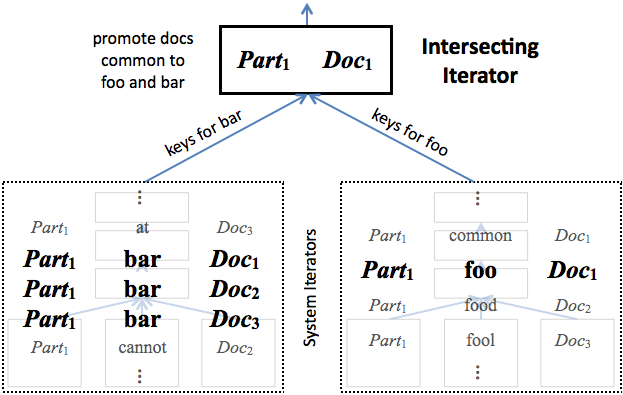
\includegraphics[width=0.8\textwidth]{images/intersecting_iterator_stack.png}
\end{center}
\end{frame}

\begin{frame}{Iterator Summary}
Iterators provide a modular implementation of Tablet Server functionality, resulting in:
\begin{itemize}
\item{Reduced complexity of Tablet Server code}
\item{Increased unit testability}
\item{Simple extensibility for specialized applications}
\end{itemize}
\end{frame}

\begin{frame}{Aggregation}
\begin{columns}
\column{.7\textwidth}

\scriptsize
Goals: Count the number of times a word appears in a dynamic corpus, and count the number of documents that contain a given word.


\begin{block}{Sample Corpus}
%\resizebox{\textwidth}{!}{
\begin{align*}
Doc_1\;:&\;\texttt{"foo and bar are common variable names"}\\
Doc_2\;:&\;\texttt{"one cannot live on bar food alone"}\\
Doc_3\;:&\;\texttt{"Mr.\noindent T pities the fool at the bar"}\\
Doc_4\;:&\;\texttt{"someone should invent the kung foo bar"}
\end{align*}
%}
\end{block}

\column{.26\textwidth}
\begin{block}{ \tiny Input Key/Value Pairs:}
\begin{center}
\resizebox{0.9in}{!}{
\begin{tabular}{|lll|}\hline
Row&Column&Value\\\hline
alone&$Doc_2$&1\\
and&$Doc_1$&1\\
are&$Doc_1$&1\\
at&$Doc_3$&1\\
bar&$Doc_1$&1\\
bar&$Doc_2$&1\\
bar&$Doc_3$&1\\
bar&$Doc_4$&1\\
cannot&$Doc_2$&1\\
common&$Doc_1$&1\\
foo&$Doc_1$&1\\
foo&$Doc_4$&1\\
food&$Doc_2$&1\\
fool&$Doc_3$&1\\
invent&$Doc_4$&1\\
kung&$Doc_4$&1\\
live&$Doc_2$&1\\
Mr.T&$Doc_3$&1\\
names&$Doc_1$&1\\
on&$Doc_2$&1\\
one&$Doc_2$&1\\
should&$Doc_4$&1\\
someone&$Doc_4$&1\\
pities&$Doc_3$&1\\
the&$Doc_3$&1\\
the&$Doc_3$&1\\
the&$Doc_4$&1\\
variable&$Doc_1$&1\\ \hline
\end{tabular}
}
\end{center}
\end{block}
\end{columns}
\end{frame}

\begin{frame}{Client Mechanisms}
\begin{itemize}
\item{BatchWriter: Group mutations and apply across the cluster in batches.}
\item{Scanner: Define a range of keys and scan sequentially through them.}
\item{BatchScanner: Execute a scan over multiple ranges in parallel.}
\end{itemize}
\end{frame}

\begin{frame}{Multiple Iterators}
\begin{columns}
\column{0.4\textwidth}
\tiny
\begin{itemize}
\item{We can compose multiple Iterators by streaming the results of one Iterator through another Iterator}
\item{Partial aggregation for the persisted view keeps the table small}
\item{Additional iterators and aggregators implement different discovery analytics at query time}
\end{itemize}
\column{0.6\textwidth}
\begin{center}
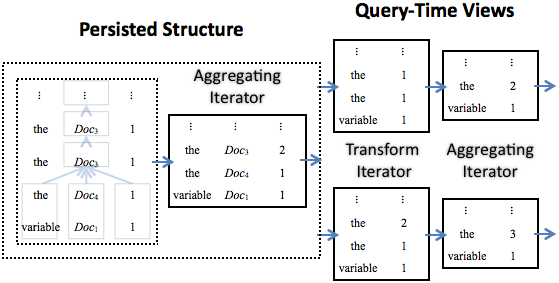
\includegraphics[width=\textwidth]{images/aggregator_complex.png}
\end{center}
\end{columns}
(MS:21 and SummingCombiner fed into SummingCombiner to get unique counts?)
\end{frame}

\section{Testing}

\begin{frame}{Accumulo VS HBase Atomic Increment}
\begin{itemize}
\item{HBase performs a server-side \emph{upsert} (read-modify-write), taking advantage of previous value being resident in write-cache}
\item{Accumulo buffers inserts and aggregates lazily but consistently, taking advantage of merge-tree data streams}
\item{Both methods implement the same atomic increment semantics}
\item{Performance varies wildly...}
\end{itemize}
\end{frame}

\begin{frame}{Performance Comparision}
\begin{columns}
\column{0.5\textwidth}
\begin{center}
Write Performance
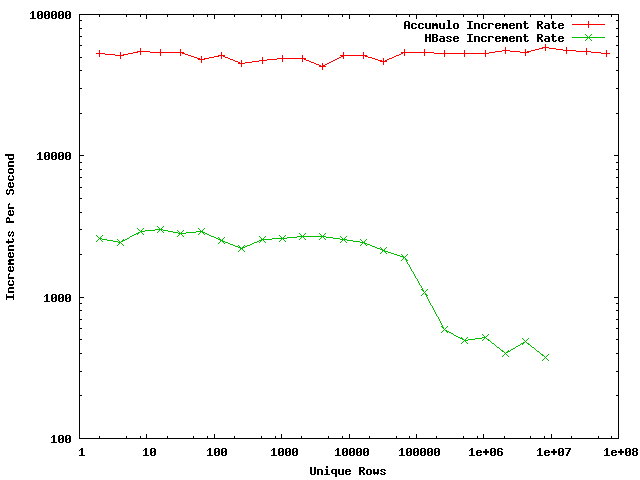
\includegraphics[width=\textwidth]{images/increment_comparison.png}
\end{center}
\column{0.5\textwidth}
\begin{center}
Read Performance
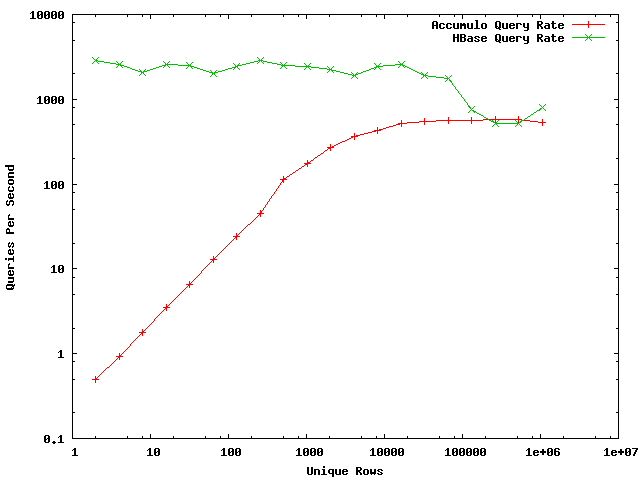
\includegraphics[width=\textwidth]{images/increment_query_comparison.png}
\end{center}
\end{columns}
\small
\begin{itemize}
\item{Aggregator wins for write performance with many different keys}
\item{Upsert wins for read performance with a small number of keys}
\item{Can we use both approaches?}
\end{itemize}
\end{frame}

\begin{frame}{Perils of Distributed Computing}
\small
Dealing with failures is hard!
\scriptsize
\begin{itemize}
\item{Operations like table creation are logically atomic, but consist of multiple operations on distributed systems.}
\item{Resource locking (via mutex, semaphores, etc.) provides some sanity.}
\item{Distributed systems have many complicated failure modes: clients, master, tablet servers, and dependent systems can all go offline periodically.}
\item{\emph{Who is responsible for unlocking locks when any component can fail?}}
\item{\emph{How do we know it's safe to unlock a lock?}}
\end{itemize}
\end{frame}

\begin{frame}{Accumulo Testing Frameworks}
\begin{itemize}
\item{\textbf{Unit}: Verify correct functioning of each module separately}
\item{\textbf{System}: Perform correctness and performance tests on a small running instance}
\item{\textbf{Load/Scale}: Generate high loads at scale and measure performance and correctness}
\item{\textbf{Random Walk}: Randomly, repeatedly, and concurrently execute a variety of test modules representative of user activity on an instance at scale}
\item{\textbf{Simulation}: Evaluate the model to gauge expected performance}
\end{itemize}
\end{frame}

\begin{frame}{Accumulo Testing Considerations}
\begin{itemize}
\item{Scoping tests to include server-side code, client-side code, dependent processes, etc.}
\item{Code coverage vs. path coverage}
\item{Static vs. dynamic analysis}
\item{Simulating failures of distributed components}
\item{Strange failure modes (often hardware/physics-related)}
\end{itemize}
\end{frame}

\begin{frame}{FATE: FAult Tolerant Executor}
\begin{itemize}
\item{If a process dies, previously submitted operations continue to execute on restart.}
\item{FATE serializes every task in Zookeeper before execution.}
\item{The Master process uses FATE to execute table operations and administrative actions.}
\item{FATE eliminates the single point of failure.}
\end{itemize}
\end{frame}

\begin{frame}[fragile]{FATE Admin Tool}
\newsavebox{\fateadmincommandbox}
\newsavebox{\fateadminbox}
\begin{lrbox}{\fateadmincommandbox}
\begin{minipage}{9in}
\color{white}
\begin{verbatim}
$ ./bin/accumulo org.apache.accumulo.server.fate.Admin print
\end{verbatim}
\end{minipage}
\end{lrbox}
\begin{lrbox}{\fateadminbox}
\begin{minipage}{9in}
\begin{verbatim}
txid: 59c0403614dc0c39 status: IN_PROGRESS op: RenameTable      locked: []     locking: [W:cz] top: RenameTable
txid: 37539f8d61548764 status: IN_PROGRESS op: ChangeTableState locked: []     locking: [W:cz] top: ChangeTableState
txid: 02f8323a3136e60d status: IN_PROGRESS op: TableRangeOp     locked: []     locking: [W:cz] top: TableRangeOp
txid: 044015732e97eec1 status: IN_PROGRESS op: CompactRange     locked: []     locking: [R:cz] top: CompactRange
txid: 6ce9dd63f9d51448 status: IN_PROGRESS op: CompactRange     locked: []     locking: [R:cz] top: CompactRange
txid: 417cb9b60e44ecd9 status: IN_PROGRESS op: TableRangeOp     locked: []     locking: [W:cz] top: TableRangeOp
txid: 5e7c5284a4677d6c status: IN_PROGRESS op: DeleteTable      locked: []     locking: [W:cz] top: DeleteTable
txid: 6633d3d841d66995 status: IN_PROGRESS op: TableRangeOp     locked: [W:cz] locking: []     top: TableRangeOpWait
\end{verbatim}
\end{minipage}
\end{lrbox}
\begin{block}{\resizebox{0.9\textwidth}{!}{\usebox{\fateadmincommandbox}}}
\resizebox{0.9\textwidth}{!}{\usebox{\fateadminbox}}
\end{block}
\scriptsize
\begin{itemize}
\item{Monitoring tool for FATE operations}
\item{Supports debugging, such as with deadlocks}
\item{Helps recovery from failed clients}
\end{itemize}
\end{frame}

\begin{frame}{FATE Summary}
\begin{columns}
\column{0.7\textwidth}
\small
\begin{itemize}
\item{FATE provides generic fault tolerance for administrative actions}
\item{With FATE, we removed custom synchronization code for a dozen procedures}
\item{Table-level locking is now low risk}
\item{Improves testability}
\item{Reduces complexity}
\item{Increases modularity}
\end{itemize}
\column{0.3\textwidth}
\tiny
\begin{block}{FATE Operations}
\begin{itemize}
\item{BulkImport}
\item{ChangeTableState}
\item{CloneTable}
\item{CompactRange}
\item{CreateTable}
\item{DeleteTable}
\item{RenameTable}
\item{TableRangeOp}
\item{DisconnectLogger}
\item{FlushTablets}
\item{ShutdownTServer}
\item{StopLogger}
\end{itemize}
\end{block}
\end{columns}
\end{frame}

\section{Design Patterns}

\begin{frame}{Design Patterns}
To use Accumulo in applications, there are several design patterns to keep in mind including:
\begin{itemize}
\item{Simple Lookup}
\item{Left-Joins From Different Sources}
\item{Null Values}
\item{Event Table w/Inverted Index}
\item{Type-agnostic Indexing}
\item{Document Partitioned Index}
\item{Multidimensional Index}
\item{Graph Index}
\end{itemize}
\end{frame}

\begin{frame}{Event Table w/Inverted Index}
\begin{center}
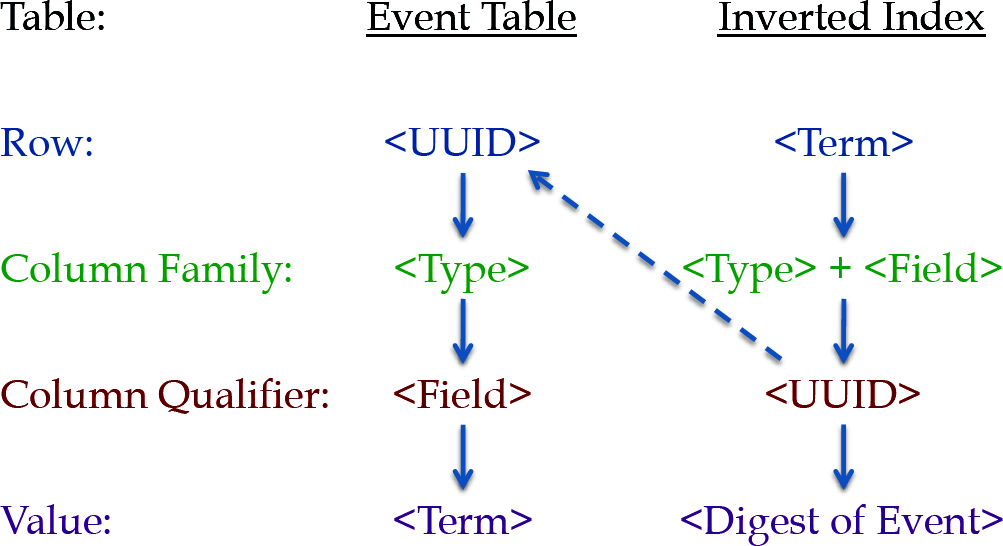
\includegraphics[width=0.9\textwidth]{images/e_ii_pattern2.png}
\end{center}
\end{frame}

\begin{frame}{Type-agnostic Indexing}
\begin{center}
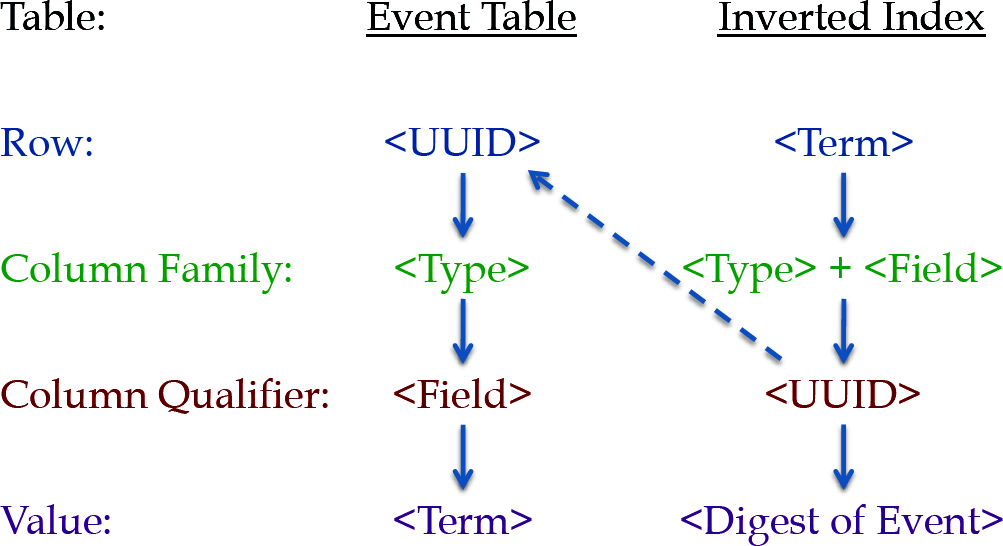
\includegraphics[width=0.9\textwidth]{images/e_ii_pattern2.png}
\end{center}
is this already covered? useful?
\end{frame}

\begin{frame}{Document Partitioned Index}
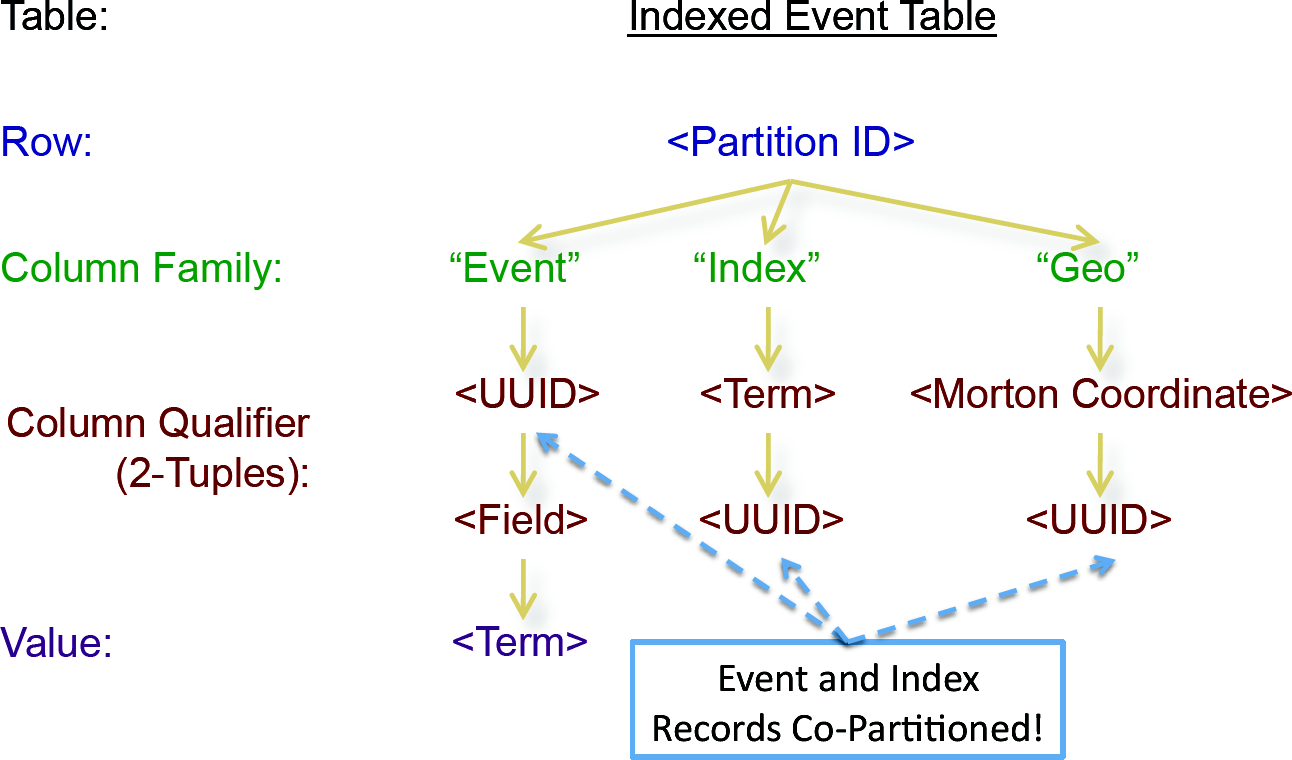
\includegraphics[width=0.9\textwidth]{images/doc_part_pattern2.png}
partition is for locality (i.e. sharding)
\end{frame}

\begin{frame}{Multidimensional Index}
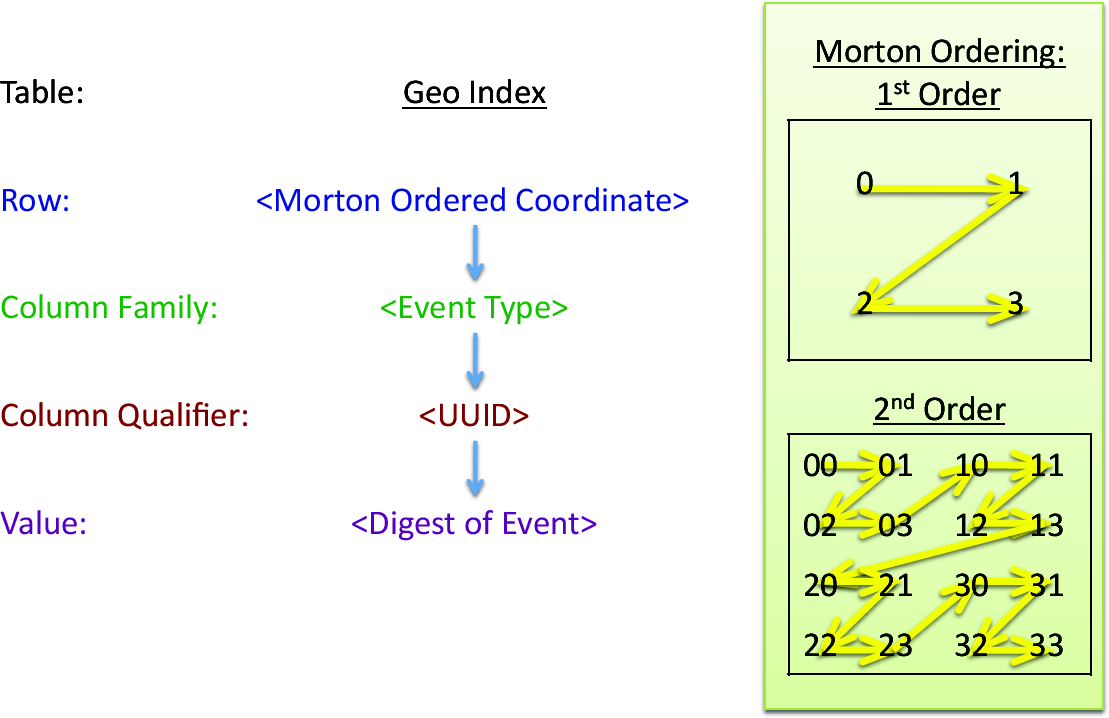
\includegraphics[width=0.9\textwidth]{images/geo_pattern.png}
\end{frame}

\begin{frame}{Graph Index}
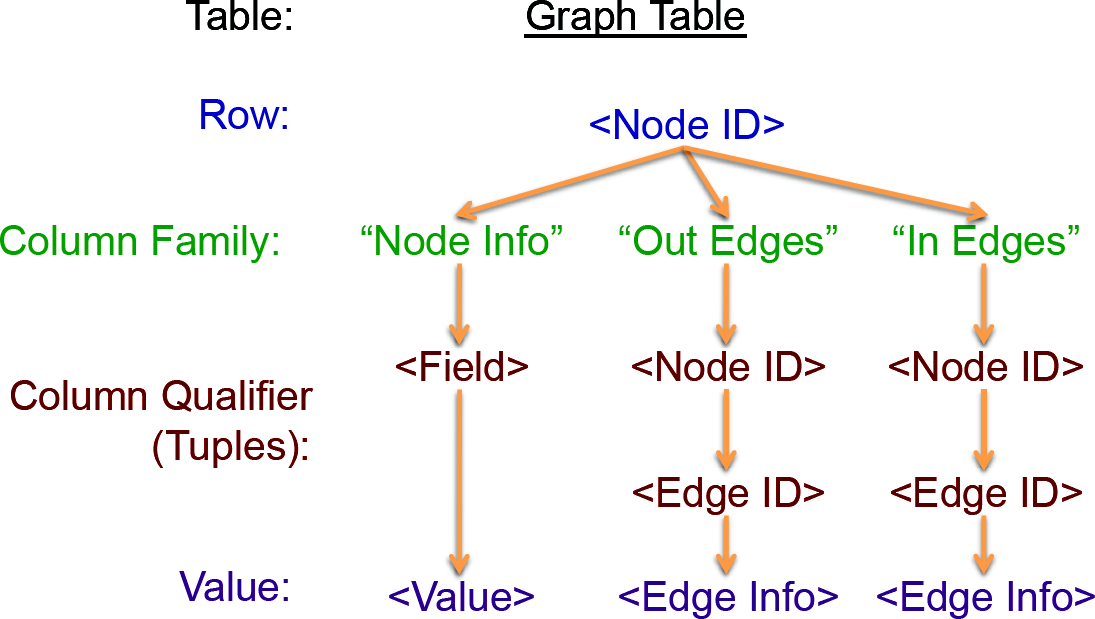
\includegraphics[width=0.9\textwidth]{images/graph_pattern2.png}
\end{frame}

\begin{frame}{Order Preserving Encodings}
\begin{columns}
\column{0.4\textwidth}
\begin{block}{Bag-O-Tricks}
\begin{itemize}
\scriptsize
\item{Subtract byte from 255 (or digit from 9) when negative}
\item{Flip signs of exponents for negative numbers}
\item{Re-order bytes based on importance}
\item{Prefix with magnitude or use fixed-precision}
\item{Unary encoding of magnitudes}
\end{itemize}
\end{block}
\column{0.6\textwidth}
\begin{itemize}
\item{Fixed precision exponent, unbounded precision significand floating point encoding: \\
{\color{red}-}{\color{blue}1.23} E{\color{green}+}{\color{orange}45} $\Rightarrow$
{\color{red}-}{\color{green}-}{\color{orange}54}{\color{blue}} {\color{blue}876}
}
\item{Variable precision integer: \\
{\color{red}12345} $\Rightarrow$ {\color{blue}11111}0{\color{red}12345}
}
\item{Tuple Encoding (no binary zero in elements): \\
{\color{red}foo},{\color{blue}bar} $\Rightarrow$ {\color{red}foo} {\textbackslash}0 {\color{blue}bar}
}
\end{itemize}
\end{columns}
\end{frame}

\begin{frame}
\frametitle{Wikipedia Search Engine Experiment}
\scriptsize
Goals:
\begin{itemize}
\item{Create a generic text indexing platform}
\item{Support a complex query language (i.e. mappable from Lucene)}
\item{Scale to multiple nodes}
\item{Support low-latency updates}
\item{Support automatic balancing and fail-over}
\end{itemize}
\begin{columns}
\column{0.5\textwidth}
\begin{block}{Data}
\begin{itemize}
\item{Three languages of Wikipedia:\\EN, ES, DE}
\item{5.9 million articles}
\item{2.37 billion (word,document) tuples}
\item{11.8 GB (compressed)}
\end{itemize}
\end{block}
\column{0.5\textwidth}
\begin{block}{Cluster}
\begin{itemize}
\item{10 Nodes}
\item{30 TB disk (60x500GB drives)}
\item{120 cores}
\item{320 GB RAM}
\end{itemize}
\end{block}
\end{columns}
\end{frame}

% MS27
\begin{frame}
\frametitle{Wikipedia Search Results}
%\begin{block}{Ingest Performance}
%TODO
%\end{block}
\scriptsize
\begin{itemize}
\item{Tested on conjunctions of high-degree terms}
\item{Retrieved entire contents of articles matching queries}
\item{Paging possible for ultra-low latency response time}
\end{itemize}
\begin{block}{Query Performance}
\scalebox{0.85}{
\tiny
\begin{tabular}{|l|l|l|l|}\hline
Query&Samples (seconds)&Matches&Result Size\\\hline
``old" and ``man" and ``sea"&\begin{tabular}{l|l|l|l|l}4.07&3.79&3.65&3.85&3.67\end{tabular}&22,956&3,830,102\\\hline
``paris" and ``in" and ``the" and ``spring"&\begin{tabular}{l|l|l|l|l}3.06&3.06&2.78&3.02&2.92\end{tabular}&10,755&1,757,293\\\hline
``rubber" and ``ducky" and ``ernie"&\begin{tabular}{l|l|l|l|l}0.08&0.08&0.10&0.11&0.10\end{tabular}&6&808\\\hline
``fast" and ( ``furious" or ``furriest")&\begin{tabular}{l|l|l|l|l}1.34&1.33&1.30&1.31&1.31\end{tabular}&2,973&493,800\\\hline
``slashdot" and ``grok"&\begin{tabular}{l|l|l|l|l}0.06&0.06&0.06&0.06&0.06\end{tabular}&14&2,371\\\hline
``three" and ``little" and ``pigs"&\begin{tabular}{l|l|l|l|l}0.92&0.91&0.90&1.08&0.88\end{tabular}&2,742&481,531\\\hline
\end{tabular}
}
\end{block}
\begin{block}{Documents per Term}
\tiny
\begin{columns}
\column{.3\textwidth}
\begin{tabular}{|l|l|}\hline
Term&Cardinality\\\hline
ducky&795\\\hline
ernie&13,433\\\hline
fast&166,813\\\hline
furious&10,535\\\hline
furriest&45\\\hline
grok&1,168\\\hline
\end{tabular}
\column{.3\textwidth}
\begin{tabular}{|l|l|}\hline
Term&Cardinality\\\hline
in&1,884,638\\\hline
little&320,748\\\hline
man&548,238\\\hline
old&720,795\\\hline
paris&232,464\\\hline
pigs&8,356\\\hline
\end{tabular}
\column{.3\textwidth}
\begin{tabular}{|l|l|}\hline
Term&Cardinality\\\hline
rubber&17,235\\\hline
sea&247,231\\\hline
slashdot&2,343\\\hline
spring&125,605\\\hline
the&3,509,498\\\hline
three&718,810\\\hline
\end{tabular}
\end{columns}
\end{block}
\end{frame}

\section{The End}

\begin{frame}{Review}
  \begin{itemize}
  \item{Accumulo can be used for a variety of applications: graph analysis, information retrieval, multi-dimensional indexing, online statistics}
  \item{Elements of all of these applications can be joined together in the same table}
  \item{Keeping the indexing separate from the database complicates the application space, but also enables new capabilities}
  \item{Use these new design patterns to build your application}
  \end{itemize}
\end{frame}

\begin{frame}{Acknowledgements}
  \begin{itemize}
  \item{This presentation was based, with permission, on Adam Fuch's slide decks. You can find the originals at http://people.apache.org/~afuchs/slides/}
  \end{itemize}
\end{frame}

\begin{frame}[c]{Questions}
  \begin{center}
  \large{Questions?}
  \end{center}
\end{frame}

\end{document}
